\documentclass[11pt,oneside,a4paper,titlepage,onecolumn]{article}

\usepackage[utf8]{inputenc}
\usepackage{textcomp}
\usepackage[official]{eurosym}
\usepackage[polish]{babel}
\usepackage{amsthm}
\usepackage{graphicx}
\usepackage[T1]{fontenc}
\usepackage{scrextend}
\usepackage{hyperref}
\usepackage{xcolor}
\usepackage{enumitem}
% \usepackage{nameref}
% \usepackage{showlabels}
% \usepackage{titlesec}
\usepackage{geometry}
\geometry{a4paper, portrait, margin=2cm}
\graphicspath{ {./fig/} }



\setcounter{secnumdepth}{4}

%% Author and title
\author{Marek Marecki \and Krzysztof Franek}
\title{%
    Proving viability of Viua VM \\
    \large Implementation of high-level language on Viua VM\\
    and deployment of simple application \\
    ~\\
    Specyfikacja Wymagań Systemowych\\
    dla czatu ViuaChat}

\begin{document}

\maketitle
{\footnotesize
\begin{center}
  \begin{tabular}{ | l | l | l | }
    \hline
    \parbox[t]{6.5cm}{\textbf{Temat pracy i akronim projektu:}\\Proving viablity of Viua VM (VVIA)} & \parbox[t]{4.5cm}{\textbf{Zleceniodawca:}\\\colorbox{yellow}{Nieznany}} & \parbox[t]{4.5cm}{\textbf{Konsultant:}\\\colorbox{yellow}{Nieznany}} \\ \hline
    \parbox[t]{6.5cm}{\textbf{Zespół projektowy:}\\Krzysztof Franek, Marek Marecki} & \parbox[t]{4.5cm}{\textbf{Kierownik projektu:}\\Marek Marecki} & \parbox[t]{4.5cm}{\textbf{Opiekun projektu:}\\dr hab. Marek A. Bednarczyk, prof. PJWSTK} \\ \hline
    \parbox[t]{3.5cm}{\textbf{Kierownik projektu:}\\Marek Marecki} & \multicolumn{2}{|l|}{\parbox[t]{9cm}{\textbf{Odpowiedzialny za dokument:}\\Krzysztof Franek}} \\ 
    \hline
  \end{tabular}
\end{center}
}

\section{Wprowadzenie}

\subsection{Cel dokumentu}
Celem dokumentu jest zdefiniowanie wymagań na podstawie analizy otoczenia aplikacji oraz analizy potrzeb projektu w stosunku do niej.

\subsection{Zakres dokumentu}
Niniejszy dokument jest produktem pierwszego etapu procesu wytwórczego czatu ViuaChat, na który składają się:
\begin{itemize}
    \item analiza otoczenia, wraz z z klientami;
    \item wskazanie kontekstu biznesowego systemu;
    \item określenie udziałowców;
	\item wyszczególnienie i uporządkowanie zasad biznesowych, jakie zostały założone w stosunku do aplikacji;
	\item opracowanie historyjek na podstawie ustalonych zasad biznesowych.
\end{itemize}

\textbf{Uwaga:} Niniejszy dokument nie dotyczy języka ViuAct ani jego kompilatora.

Praca wygenerowana w systemie \LaTeX.

\subsection{Dokumenty powiązane}
\begin{itemize}
	\item Szkic funkcjonalności ViuaChat - pierwszy zarys zasad biznesowych, ujęty w formie prostego konspektu;
	\item Specyfikacja wymagań biznesowych i \textit{user stories} - starsza wersja dokumentu SWS, nieujmująca otoczenia i kontekstu aplikacji.
\end{itemize}

\subsection{Odbiorcy}
Dokument został skierowany przede wszystkim dla członków zespołu, aby ułatwić im współpracę - w szczególności wówczas, gdy funkcjonalności czatu mogą pociągać za sobą modyfikację zestawu bibliotek ViuaVM bądź struktury składni projektowanego języka ViuAct.

Kolejną grupą adresatów niniejszego dokumentu są pracownicy uczelni, odpowiedzialni za nadzór nad prawidłowym ukształtowaniem i przebiegiem projektu. Wśród nich, szczególną rolę odgrywa JE Dziekan ZWI, prof. Marek Bednarczyk, będący opiekunem projektu.

\subsection{Słownik pojęć}
\begin{description}
  \item[Pokój] Współdzielony czat, do którego dostęp ma równocześnie wielu uczestników, widzących nawzajem wysyłane przez siebie wiadomości
  \item[Wpięcie użytkownika w pokój] Rodzaj relacji, polegający na tym, że dany użytkownik ma możliwość nadawania i odbierania wiadomości w ramach określonego pokoju
  \item[Użytkownik tymczasowy] Typ użytkownika, którego konto jest tworzone podczas połączenia z serwerem czatu oraz niszczone po jego zakończeniu
  \item[Użytkownik stały] Typ użytkownika, którego konto jest utrzymywane przez serwer pomiędzy połączeniami do czatu
  \item[Wiadomości prywatne] Wiadomości, które są wysyłane konkretnemu użytkownikowi i są widoczne wyłącznie dla nadawcy i odbiorcy takiej wiadomości
  \item[ViuAct] Język programowania wysokiego poziomu, oparty o model aktorów, powstały na potrzeby niniejszego projektu inżynierskiego
\end{description}

\section{Czat w kontekście}

\subsection{Kontekst biznesowy}

Niniejszy czat stanowi część szerszego kontekstu, jakim jest potrzeba zademonstrowania działania języka ViuAct oraz całego środowiska wytwórczego powiązanego z maszyną wirtualną ViuaVM.

\begin{figure}[h]
	\centering
	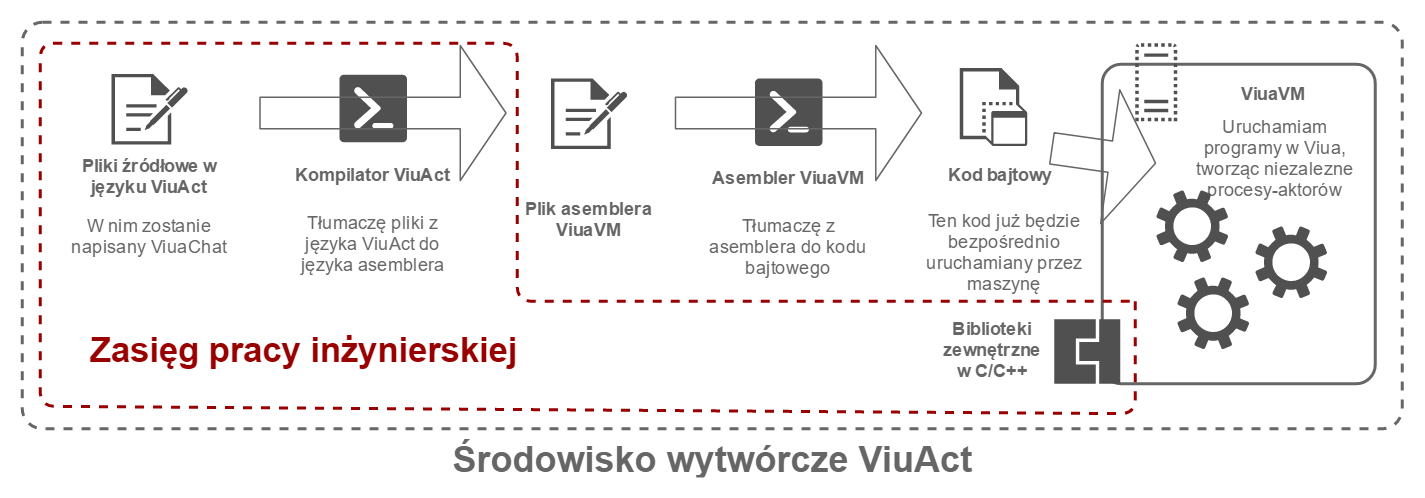
\includegraphics[width=\textwidth]{viuavm-env}
	\caption{Ilustracja środowiska wytwórczego wraz zasięgiem, którym są objęte prace przewidziane projektem inżynierskim}
\end{figure}

Cel demonstracyjny jest pierwszym i najważniejszym, jaki przyświeca konstrukcji czatu. Ponadto, sam proces wytwórczy pozwoli
przetestować wydajność całego środowiska w jego praktycznym wymiarze. Tym samym, możliwe będzie poprawienie konstrukcji kompilatora 
lub zastosowanych konstrukcji językowych ViuAct, podnoszących jego użyteczność.

Wszelcy odbiorcy dla aplikacji czatu zostaną, podobnie jak sama aplikacja, skonstruowani na cele demonstracyjne. Nie powinni oni
odbiegać od modelowych odbiorców podobnych komunikatorów, tak, aby potencjalny, poczatkujący użytkownik środowiska ViuaVM mógł
zrozumieć intencje stojące za rozwiązaniami zastosowanymi w ViuaChat oraz przenieść je do swoich pierwszych programów, opracowanych
w tym środowisku.

\subsection{Udziałowcy}
\textit{Udziałowiec to każdy podmiot, ożywiony bądź nie (osoba, system, urządzenie, regulacje prawne, społeczeństwo itp), który bierze udział w projekcie, lub na którego projekt może wpływać.
Dla projektów, które powstają w oparciu o istniejącą infrastrukturę techniczną, należy pamiętać o włączeniu tej infrastruktury jako udziałowca nieożywionego, którego istnienie narzuca pewne rozwiązania i wymagania}

  \begin{tabular}{ | l | l | }
  
	\hline
	\multicolumn{2}{ | l | }{\textbf{Karta udziałowca}}  \\
  
	\hline
    \parbox[t]{4cm}{
    	\textbf{Identyfikator}
    } & UN-01 \\  
    
    \hline
    \parbox[t]{4cm}{
    	\textbf{Nazwa}
    } & ViuaVM \\  
    
    \hline
    \parbox[t]{4cm}{
    	\textbf{Opis}
    } & Środowisko, o które opiera się projekt... \\ 
    
    \hline
    \parbox[t]{4cm}{
    	\textbf{Typ}
    } & Nieożywiony, bezpośredni \\  
    
    \hline
    \parbox[t]{4cm}{
    	\textbf{Punkt widzenia}
    } & Punkt widzenia... \\ 
    
    \hline
    \parbox[t]{4cm}{
    	\textbf{Ograniczenia}
    } & Ograniczenia... \\ 
    
    \hline
    \parbox[t]{4cm}{
    	\textbf{Wymagania}
    } & O-1... \\ 
  
    \hline
  \end{tabular}

\subsection{Klienci}

\textit{Klienci wewnętrzni są to klienci, którzy występują w ramach naszej organizacji np. nasz szef, dział finansowy, konstruktorzy, instalatorzy itp. specyfikujemy ich charakterystykę i potrzeby w odniesieniu do naszego projektu.
Klienci zewnętrzni - przedstawiciele zleceniodawcy, którzy mogą mieć bardzo różne potrzeby np. dyrektor i administrator sieci, za klientów zewnętrznych uważa się także podwykonawców i dostawców.}

\subsection{Charakterystyka użytkowników}

\textit{Użytkownicy, ich kategorie, uprawnienia dostępu do funkcji i danych w poszczególnych trybach pracy systemu; zakładana liczebność użytkowników poszczególnych kategorii}

\subsection{Istniejąca infrastruktura}

\textit{Inwentaryzacja istniejącej infrastruktury z zaznaczeniem, co należy zastąpić, a co należy wykorzystać w systemie, o ile użytkownik nie zostawia tego do decyzji projektanta rozwiązania technicznego. Może być przedstawiona w tabeli lub punktach.}

\section{Wymagania}

\subsection{Zasady biznesowe}

Zidentyfikowane zasady pogrupowano w 3 kategorie, biorąc pod uwagę podstawowe bloki funkcjonalności. Przydzielenie
do kategorii jest sygnalizowanie literą alfabetu, będącą prefiksem identyfikatora danej zasady. Dokonano
również priorytetyzacji zasad biznesowych według klasycznej skali ,,MoSCoW":

\begin{itemize}
	\item \textbf{,,M''} (z ang. \textit{must}) - zasady, których spełnienie jest niezbędne dla realizacji systemu
	\item \textbf{,,S''} (z ang. \textit{should}) - są to zasady o wysokim priorytecie, które powinny;
	zostać spełnione, o ile tylko jest to możliwe;
	\item \textbf{,,C''} (z ang. \textit{could}) - dobrze byłoby zrealizować takie wymagania, ale zależy to od czasu
	i zasobów, jakie pozostaną do dyspozycji po ukończeniu zadań ,,M" i ,,C";
	\item \textbf{,,W''} (z ang. \textit{won't}) - takie wymagania, po dyskusji, zostały wycofane dalszej realizacji.
\end{itemize}

\subsubsection{System użytkowników [U]}
  \begin{tabular}{ | l | l | l | }
	\hline
    \textbf{ID} & \parbox[t]{14cm}{
    	\textbf{Zasada biznesowa}
    } & \textbf{Priorytet} \\  
  
    \hline
    U-1 & \parbox[t]{14cm}{
      Podczas wejścia na czat, użytkownikowi pokazuje się monit z polem do wpisania nazwy użytkownika. 
    } & M \\

    \hline
    U-2 & \parbox[t]{14cm}{
      Użytkownicy bez stałego konta podczas logowania podają tylko nazwę użytkownika, pole hasła pozostaje puste .
    } & M \\

    \hline
    U-3 & \parbox[t]{14cm}{
      Nazwa użytkownika to ciąg od 3 do 32 alfanumerycznych znaków.
    } & M \\

    \hline
    U-4 & \parbox[t]{14cm}{
      Można rozpocząć sesję jako użytkownik, pod warunkiem, że zadeklarowana nazwa nie będzie powtarzać się z nazwami już zalogowanych użytkowników. 
    } & M \\

    \hline
    U-5 & \parbox[t]{14cm}{
      Monit podczas wejścia na czat jest wyposażony w pole do wpisania hasła (nieobowiązkowe). 
    } & S \\

    \hline
    U-6 & \parbox[t]{14cm}{
      Użytkownicy czatu ze stałym kontem, podczas logowania podają nazwę i odpowiadające mu hasło.
    } & S \\

    \hline
    U-7 & \parbox[t]{14cm}{
      Stałe konta użytkowników są utrzymywane na serwerze w postaci trójek wartości: nazwa użytkownika, hasło (md5), czy jest administratorem. 
    } & S \\

    \hline
    U-8 & \parbox[t]{14cm}{
      Nie można rozpocząć sesji użytkownika o nazwie, która pasuje do istniejącego konta, jeżeli nie zostanie podane prawidłowe hasło (nie można podszywać się pod nazwy użytkowników ze stałym kontem).
    } & S \\

    \hline
    U-9 & \parbox[t]{14cm}{
      Można rozpocząć sesję jako użytkownik bez podawania hasła, pod warunkiem, że zadeklarowana nazwa nie będzie powtarzać się z nazwami stałych kont użytkowników.
    } & S \\

    \hline
    U-10 & \parbox[t]{14cm}{
      W okienkach czatu, loginy użytkowników ze stałym kontem są pogrubione i pokolorowane: Administratorzy na czerwono,
      Pozostali na zielono. 
      } & S \\

    \hline
    U-11 & \parbox[t]{14cm}{
      Administratorzy mają prawo przeglądać nazwy pokojów na serwerze. 
    } & M \\

    \hline
    U-12 & \parbox[t]{14cm}{
      Administratorzy mają prawo tworzyć i usuwać pokoje. 
    } & S \\

    \hline
    U-13 & \parbox[t]{14cm}{
      Administratorzy mają prawo ustanawiać, zmieniać i usuwać hasła do pokojów. 
    } & C \\

    \hline
    U-14 & \parbox[t]{14cm}{
      Administratorzy mają prawo wyrzucać użytkowników z pokojów. 
    } & C \\

    \hline
    U-15 & \parbox[t]{14cm}{
      Administratorzy mają prawo wyrzucać użytkowników z serwera. 
    } & C \\

    \hline
    U-16 & \parbox[t]{14cm}{
      Administratorzy mają prawo przeglądać nazwy i poziomy uprawnień kont stałych użytkowników. 
    } & M \\

    \hline
    U-17 & \parbox[t]{14cm}{
      Administratorzy mają prawo tworzyć i usuwać użytkowników. 
    } & S \\

    \hline
    U-18 & \parbox[t]{14cm}{
      Administratorzy mają prawo zmieniać hasła użytkowników. 
    } & C \\

    \hline
    U-19 & \parbox[t]{14cm}{
      Administratorzy mają prawo zmieniać uprawnienia stałych kont użytkowników. 
    } & C \\

    \hline
    U-20 & \parbox[t]{14cm}{
      Użytkownicy ze stałymi kontami mogą zmieniać swoje hasło.
    } & W \\

    
    \hline
  \end{tabular}

\subsubsection{Pokoje [P]}
  \begin{tabular}{ | l | l | l | }
	\hline
    \textbf{ID} & \parbox[t]{14cm}{
    	\textbf{Zasada biznesowa}
    } & \textbf{Priorytet} \\  
    
    \hline
    P-1 & \parbox[t]{14cm}{
      Pokoje to właściwe czaty – tam użytkownicy mogą wejść i pisać do siebie nazwajem
    } & M \\

    \hline
    P-2 & \parbox[t]{14cm}{
      Każdy pokój ma unikalną nazwę będącą ciągiem alfanumerycznym od 3 do 32 znaków
    } & M \\

    \hline
    P-3 & \parbox[t]{14cm}{
      Lista pokojów jest widoczna dla każdego użytkownika po zalogowaniu się do serwera czatu
    } & M \\

    \hline
    P-4 & \parbox[t]{14cm}{
      Użytkownik może być równocześnie wpięty do jednego pokoju
    } & M \\

    \hline
    P-5 & \parbox[t]{14cm}{
      Wiadomość wysłana w pokoju jest widoczna w oknie pokoju dla wszystkich użytkowników podpiętych do tego pokoju
    } & M \\

    \hline
    P-6 & \parbox[t]{14cm}{
      Użytkownik może się samodzielnie wypiąć z pokoju, do którego jest wpięty
    } & S \\

    \hline
    P-7 & \parbox[t]{14cm}{
      Pokój może mieć ustanowione hasło, które użytkownik musi wpisać przed podpięciem się do niego
    } & C \\
    
    \hline
    
  \end{tabular}

\subsubsection{Prywatne wiadomości [W]}
  \begin{tabular}{ | l | l | l | }
  	\hline
    \textbf{ID} & \parbox[t]{14cm}{
    	\textbf{Zasada biznesowa}
    } & \textbf{Priorytet} \\  
    
    
    \hline
    W-1 & \parbox[t]{14cm}{
      Oprócz okien czatu dla każdego z wpiętych pokojów, użytkownik dysponuje dodatkowym oknem, na którym widzi wiadomości prywatne. 
    } & M \\

    \hline
    W-2 & \parbox[t]{14cm}{
      Aby wysłać wiadomość prywatną, należy poprzedzić ją znakiem \# i nazwą użytkownika, do którego jest kierowana wiadomość, oddzielona spacją od komunikatu, np.: „\#user Tajna wiadomość”. Trafia ona wówczas do okna wiadomości prywatnych. 
    } & M \\

    \hline
    W-3 & \parbox[t]{14cm}{
      Wiadomość prywatna może być wysłana z okna czatu pokoju –wiadomości prywatne nie są pokazywane wszystkim uczestnikom czatu, a jedynie użytkownikowi, do którego jest adresowana. 
    } & C \\

    \hline
    W-4 & \parbox[t]{14cm}{
      W oknie czatu pokoju dopuszczalne jest wysyłanie wiadomości prywatnych do dowolnych użytkowników, nawet tych, którzy nie są w danym momencie podpięci do tego pokoju. 
    } & C \\

    \hline
    W-5 & \parbox[t]{14cm}{
      Z okna wiadomości prywatnych można wysyłać wyłącznie wiadomości prywatne. 
    } & M \\

    \hline
    W-6 & \parbox[t]{14cm}{
      Próba wysłania wiadomości prywatnej powinna zostać odrzucona przez serwer i zwrócić błąd w przypadku gdy:
      \begin{itemize}
      	\item Po znaku „\#” pojawi się od razu znak spacji lub nie będzie żadnych znaków (nie zostanie podana 
		nazwa użytkownika który jest adresatem)
		\item Nazwa adresata jest dłuższa niż 32 znaki
		\item Na serwerze nie istnieje użytkownik z nazwą użytą jako nazwa adresata
		\item Adresat wiadomości ma swoje konto na serwerze, ale nie jest zalogowany 
      \end{itemize}
		
    } & M \\
    \hline
    
  \end{tabular}


\subsection{Historyjki (\textit{user stories})}

\begin{tabular}{ | l | l | }
	\hline
		\textbf{Identyfikator} & 
		HF-1
		\\
		
	\hline
		\textbf{Treść} & \parbox[t]{13cm}{
			Jako użytkownik serwera czatu, chcę móc się do niego zalogować, aby zobaczyć listę pokojów dyskusyjnych.
		}\\
		 
	\hline
		\parbox[t]{4cm}{\textbf{Powiązane zasady biznesowe}} & \parbox[t]{13cm}{
			U-1 Podczas wejścia na czat, użytkownikowi pokazuje się monit z polem do wpisania nazwy użytkownika.
		}\\
		
	\hline
		\parbox[t]{4cm}{\textbf{Kryteria akceptacji}} & \parbox[t]{13cm}{
			\begin{enumerate}
				\item Po wejściu na czat bez rozpoczętej sesji, pokazuje się monit o podanie nazwy użytkownika.
				\item Po wpisaniu nazwy użytkownika i zatwierdzeniu, użytkownik rozpocznie sesję na serwerze czatu.
				\item Tuż po rozpoczęciu sesji czatu, użytkownik zobaczy listę pokojów.
			\end{enumerate}
			}
		\\

	\hline
\end{tabular}

\textit{Tu muszą zostać przeklejone karty z Trello}

\subsection{Wymagania niefunkcjonalne}

\begin{tabular}{ | l | l | }
	\hline
		\textbf{Identyfikator} & 
		HN-1
		\\
		
	\hline
		\textbf{Treść} & \parbox[t]{13cm}{
			Długość nazwy użytkownika jest ograniczona od 2 do 32 znaków alfanumerycznych, w celu uniknięcia problemów z identyfikacją użytkownika na serwerze.
		}\\
		 
	\hline
		\parbox[t]{4cm}{\textbf{Powiązane zasady biznesowe}} & \parbox[t]{13cm}{
			U-3 Nazwa użytkownika to ciąg od 3 do 32 alfanumerycznych znaków.
		}\\
		
	\hline
		\parbox[t]{4cm}{\textbf{Kryteria akceptacji}} & \parbox[t]{13cm}{
			\begin{enumerate}
				\item Po wpisaniu do pola użytkownika nazwy krótszej niż 2 znaki, dłużej niż 32 znaki lub zawierającej inne znaki niż alfanumeryczne, zwracany jest błąd.
			\end{enumerate}
			}
		\\

	\hline
\end{tabular}

\textit{Tu muszą zostać przeklejone karty z Trello}

\subsection{Wymagania na środowisko docelowe}

\textit{W jakim środowisku będzie pracować system – o ile jest istotne, np. system operacyjny, rodzaje i wersje przeglądarek internetowych, itp. Może się zdarzyć, że na tym etapie użytkownicy i inni udziałowcy nie wyspecyfikują środowiska docelowego.}

\subsection{Wymagania dotyczące procesu wytwarzania}

\textit{Jaki ma być proces powstawania rozwiązania projektowego np. ile czasu ma trwać, czy ma być wykonany zgodnie z jakąś metodologią lub też jakie mają być cechy tego procesu np. tajny}

\section{Kryteria akceptacja rozwiązania}

\textit{Specyfikacja kryteriów akceptacji gotowego produktu przez klienta – mogą to być wybrane kluczowe wymagania funkcjonalne lub niefunkcjonalne. Chodzi o zdefiniowanie priorytetów: czas, budżet, wydajność, bezpieczeństwo, itp. Pod koniec procesu realizacji wraca się do kryteriów akceptacji zdefiniowanych na początku projektu i weryfikuje poprawność rozwiązania. }

\section{Odwołania do literatury}

\textit{Lista przywoływanych pozycji literowych, ponumerowanych lub z przydzielonymi identyfikatorami; w treści właściwej dokumentu posługujemy się wyłącznie numerami/ identyfikatorami do wskazania źródła treści. Usunąć jeśli nie dotyczy.}

\end{document}
